\chapter{Complexity Factors}
\label{ch:unmaintainability}

After analysing the different approaches taken by previous work, we define a number of requirements and challenges our solution will have to meet and overcome. Most of these generate complexity in the system, and make for potential issues for long term support of such a system. As such, starting with the analysis of these issues, we focus our attention on the maintainability issues related with this project.

\section{Generality}

To lower the coupling between our software and \acrshort{vtk}, we want it to be version-agnostic. This coupling is already weakened by the fact the library is developed to be backwards-compatible and the only major change to the API that broke this happened between versions 4 and 6 of the library\footnote{https://vtk.org/Wiki/VTK/VTK\_6\_Migration/Overview}. 

We further aim at enabling the user to use the library to its full potential, limiting the components that cannot be reached from within the development environment and that require technical knowledge to be integrated through code. As we discussed in Section~\ref{sec:related-work}, both the OculusVTK implementation by Dreuning and the ActiViz plugin have this capability. However, the first is limited to Python and using OculusVR supported \acrshort{hmd}s, whereas the second is limited by its performances. 

Hardcoding \acrshort{vtk}s features would make for the best performances, but would make the system plugin a huge collection of functions, as it would be necessary to wrap the calls for every class and method accessible to the user. This approach would potentially be the more performant, but makes for a hardly maintainable system.

Instead, our approach aims to integrate Dreuning's Python introspection scripts within a C++ native plugin, as this would still allow for a performing system written in C++ to access Python's capabilities when it is necessary to expose parts of \acrshort{vtk} the system has no direct access to.

Introducing these Python scripts within the C++ plugin can be achieved through two different approaches: keeping the Python component separate and make it communicate with the C++ native plugin or embedding the Python interpreter within the C++ code itself. 

Although the first option would make for better separation of concerns, it introduces a non-trivial issue with memory sharing, synchronization and performance, as the two parts would need to communicate, both should be able to read and write the \acrshort{vtk} objects being handled and this should be executed in a timely fashion. These operations, although can achieve the required performances of completing a full cycle in around 11.1 ms (90 \acrshort{fps} for most \acrshort{hmd}s is the recommended refresh rate), comprising of updating both lenses' views, requires careful crafting and optimizing, introducing design and code complexity.

On the other hand, the embeding of the Python interpreter is a common choice and is discussed in the official guidelines of Python itself\footnote{\url{https://docs.python.org/3/extending/embedding.html}} and can achieve decent performances. In order to determine the overhead introduced by the embedding, we compare the execution times of an embedded application with the same application in pure Python and repeat this for direct access to \acrshort{vtk} and using the Dreuning's introspection scripts.s

The application we run is a stream tracer of a density dataset for \acrshort{vtk} applications. The final visualization is composed of the outline and the streamlines. The pipeline can be seen in Figure~\ref{fig:streamtracer_pipeline}.

\begin{figure}
    \centering
    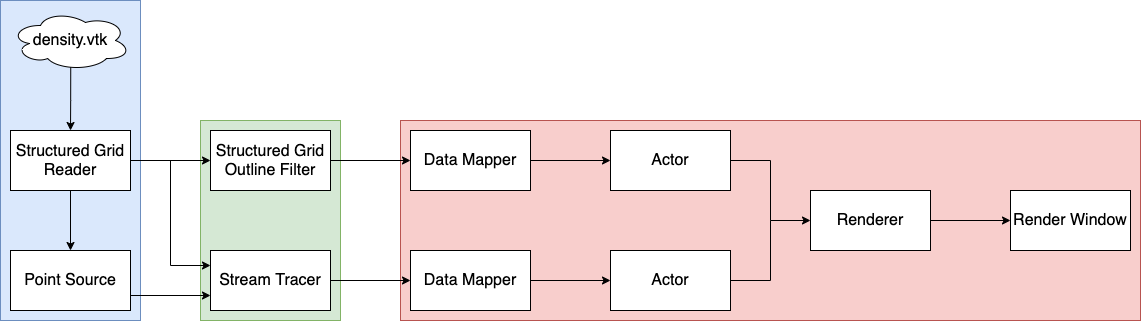
\includegraphics[width=\textwidth]{pictures/streamtracer_pipeline.png}
    \caption{VTK pipeline of a Stream Tracer on a density dataset.}
    \label{fig:streamtracer_pipeline}
\end{figure}